\section{Casi d'uso}

	\subsection{Introduzione}
Il numero limitato dei casi d'uso\glo identificati è dovuto alla natura del prodotto, in quanto si tratta di un plug-in e quindi di un'estensione di una piattaforma già esistente che viene integrata da un tool di addestramento esterno.
Per la piattaforma in questione non è fornita alcuna documentazione in quanto essa è già disponibile al sito web del distributore della piattaforma: \emph{Grafana Labs} (\href{https://grafana.com/docs/grafana/latest/}{Grafana Documentation}).

	\subsection{Struttura}
Viene riportata di seguito la classificazione dei casi d'uso. Verranno descritti nel documento rispettando la struttura esposta di seguito.
		\begin{itemize}
			\item codice identificativo;
			\item titolo;
			\item diagramma UML (se presente);
			\item attore primario;
			\item precondizioni;
			\item postcondizioni;
			\item scenario principale;
			\item estensioni (se presenti);
			\item inclusioni (se presenti).
		\end{itemize}
Verrà utilizzato il linguaggio di modellazione UML 2.0\glo.
Ogni requisito può essere inserito in vari UC\glo, che si differenziano ciascuno per una diversa profondità dei dettagli da cui possono distinguersi ulteriori requisiti.

\subsection{Classificazione}
Identificare i casi d'uso in modo univoco aiuta la tracciabilità. I casi d'uso sono classificati nel seguente modo: \\
\centerline{\textbf{UC[codice\_padre].[codice\_figlio]}} \\
Il \textit{codice\_padre} è il codice univoco che rappresenta il requisito del caso d'uso. Se lo UC è collegato per profondità di dettaglio ad un altro UC, il \textit{codice\_figlio} verrà rappresentato in maniera gerarchica (esempio: se uno UC rappresenta un livello di dettaglio maggiore con \textit{codice\_padre} x, il suo codice sarà x.y, dove y indica l'annidamento raggiunto). \\ Verranno presentati prima i casi d'uso principali (da \hyperref[par:UC1]{UC1} a \hyperref[par:UC8]{UC8}), seguiti da quelli relativi ad estensioni (da \hyperref[par:UC9]{UC9} a \hyperref[par:UC24]{UC24}).

	\subsection{Attori}
Il sistema di autenticazione e registrazione dell'utente viene gestito per intero dal sistema Grafana, in quanto il prodotto finale non disporrà di una funzionalità di autenticazione/registrazione interna.									
Il numero limitato di differenti attori che si approcciano a parte del prodotto in analisi è dovuto principalmente al fatto che, essendo il prodotto \emph{Predire in Grafana} costituito da un plug-in del sistema indipendente di Grafana ed un tool di addestramento, un esiguo numero di utenti hanno effettivamente la possibilità di approcciarsi al monitoraggio dei dati.
Per poter usare al meglio il tool di addestramento è consigliabile che l'utente disponga di nozioni di Machine Learning. Per sfruttare al meglio il plug-in si raccomanda conoscenza riguardo il monitoraggio dei dati e di saper interpretare le previsioni visualizzate sulla dashboard. 
Inoltre non è necessaria la  registrazione degli utenti poiché l'addestramento avviene in un tool esterno.


	\subsubsection{Attori primari}
Essendo il prodotto finale un plug-in open-source\glo è accessibile ad ogni tipo di utente. L'attore primario individuato è l'utente generico.
	\subsubsection{Attori secondari}
	\begin{itemize}
		\item\textbf{Piattaforma Grafana}: è un sistema di monitoraggio di stream\glo di dati, che ospiterà il plug-in prodotto. Consente agli utenti registrati di lanciare alert e realizzare grafici modellati sui dati forniti in ingresso al plug-in.
	\end{itemize}

% - Casi d'uso: Principali - %%%%%%%%%%%%%%%%%%%%%%%%%%%%%%%%%%%

	\label{par:UC1}
	\subsection{UC1 - Creazione file JSON dai dati di addestramento}

	\begin{figure}[H]
		\centering
		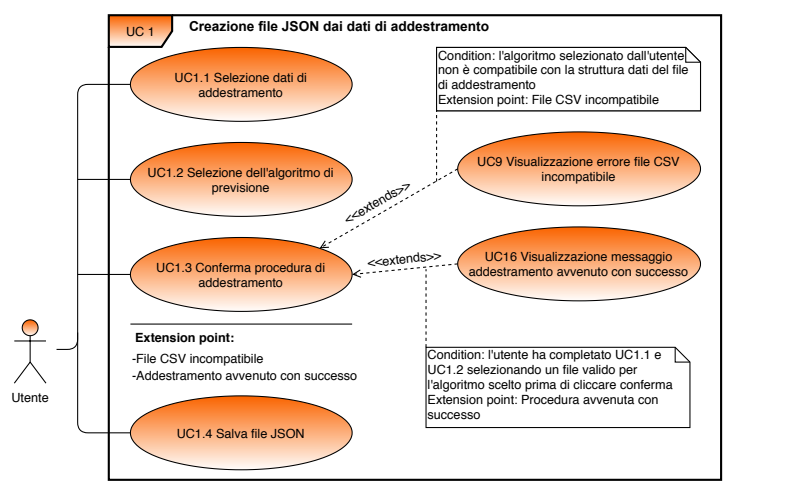
\includegraphics[scale=0.70]{../Analisi_dei_requisiti/img/Diagrammi_UML/UC1_tool_di_addestramento.png}
		\caption{Creazione file JSON dai dati di addestramento}
	\end{figure}	

		\begin{itemize}
			\item\textbf{Attore primario}: utente generico;
			\item\textbf{Precondizioni}:
				\begin{enumerate}
					\item l'utente deve possedere dei dati di addestramento\glo in un file formato CSV\glo;
					\item l'utente si trova sulla pagina web dedicata al tool di addestramento.
				\end{enumerate}
			\item\textbf{Postcondizioni}:
				\begin{enumerate}
					\item viene addestrato l'algoritmo in base al CSV inserito;
					\item l'utente ha prodotto il file JSON contenente i predittori dell'algoritmo addestrato.
				\end{enumerate}
			\item\textbf{Scenario principale}:
				\begin{enumerate}
					\item (\hyperref[par:UC1.1]{UC1.1}) l'utente seleziona i dati di addestramento da caricare;
					\item (\hyperref[par:UC1.2]{UC1.2}) l'utente seleziona l'algoritmo di previsione scelto attraverso la Combo Box\glo “Scegli algoritmo”;
					\item (\hyperref[par:UC1.3]{UC1.3}) conferma delle operazioni;
					\item (\hyperref[par:UC1.4]{UC1.4}) viene visualizzato a schermo un messaggio di notifica di avvenuto successo della procedura di addestramento se tutto è stato eseguito correttamente;
					\item (\hyperref[par:UC1.5]{UC1.5}) viene visualizzato a schermo un messaggio di alert addestramento non riuscito se si sono verificati imprevisti durante la procedura di addestramento;
					\item (\hyperref[par:UC1.6]{UC1.6}) l'utente scarica l'addestramento ricevendo in output il file JSON contenente i predittori per SVM/RL che viene salvato localmente.
				\end{enumerate}
			\item\textbf{Estensioni}: 
				\begin{enumerate}
					\item \hyperref[par:UC7]{UC7} estende \hyperref[par:UC1.3]{UC1.3}: viene visualizzato un messaggio d'errore se non è stato caricato alcun file CSV contenente i dati di addestramento;
					\item \hyperref[par:UC8]{UC8} estende \hyperref[par:UC1.3]{UC1.3}: viene visualizzato un messaggio d'errore se non è stato scelto alcun algoritmo per l'addestramento;
					\item \hyperref[par:UC9]{UC9} estende \hyperref[par:UC1.3]{UC1.3}: viene visualizzato un messaggio d'errore se il file di addestramento è incompatibile con l'algoritmo scelto.
				\end{enumerate}
			
		\end{itemize}
		
		\label{par:UC1.1}
		\subsubsection{UC1.1 - Selezione dati di addestramento }
		\begin{itemize}
			\item\textbf{Attore primario}: utente generico;
			\item\textbf{Precondizioni}:
				\begin{enumerate}
					\item l'utente si trova sulla pagina web dedicata al tool di addestramento;
					\item l'utente deve possedere il file CSV;
					\item l'utente deve aver cliccato il pulsante di caricamento dati di addestramento.
				\end{enumerate}
			\item\textbf{Postcondizioni}: l'utente ha selezionato il file dei dati di addestramento;
			\item\textbf{Scenario principale}: l'utente seleziona il file CSV contenente i dati di addestramento dal file system ed è visibile solo il formato CSV.
		\end{itemize}
		
		\label{par:UC1.2}
		\subsubsection{UC1.2 - Selezione dell'algoritmo di previsione}
		\begin{itemize}
			\item\textbf{Attore primario}: utente generico;
			\item\textbf{Precondizioni}: l'utente deve aver selezionato i dati di addestramento (\hyperref[par:UC1.1]{UC1.1});
			\item\textbf{Postcondizioni}: l'utente ha scelto l'algoritmo di previsione selezionando l'opzione corrispondente;
			\item\textbf{Scenario principale}: l'utente clicca la Combo Box con etichetta "Seleziona Algoritmo" e sceglie l'algoritmo da addestrare (Support Vector Machine o Regressione Lineare).
		\end{itemize}
	
	\label{par:UC1.3}
	\subsubsection{UC1.3 - Conferma procedura addestramento}
		\begin{itemize}
			\item\textbf{Attore primario}: utente generico;
			\item\textbf{Precondizioni}:
				\begin{enumerate}
					\item l'utente deve aver caricato i dati di addestramento (\hyperref[par:UC1.1]{UC1.1});
					\item l'utente deve aver selezionato l'algoritmo che vuole utilizzare per la previsione (\hyperref[par:UC1.2]{UC1.2}).
				\end{enumerate}
			\item\textbf{Postcondizioni}:
				\begin{enumerate}
					\item l'utente ha confermato la scelta dell'algoritmo e l'inserimento dei dati di addestramento;
					\item l'utente ha addestrato l'algoritmo e può scaricare il file JSON.
				\end{enumerate}
			\item\textbf{Scenario principale}: l'utente clicca il pulsante con etichetta “Conferma”;
			\item\textbf{Estensioni}:
			\begin{enumerate}
				\item \hyperref[par:UC7]{UC7}: viene visualizzato un messaggio d'errore se non è stato caricato alcun file CSV contenente i dati di addestramento;
				\item \hyperref[par:UC8]{UC8}: viene visualizzato un messaggio d'errore se non è stato scelto alcun algoritmo per l'addestramento;
				\item \hyperref[par:UC9]{UC9}: viene visualizzato un messaggio d'errore se il file di addestramento è incompatibile con l'algoritmo scelto.
			\end{enumerate}
			 
						
		\end{itemize}
		
	\label{par:UC1.4}
	\subsubsection{UC1.4 - Visualizzazione messaggio di notifica "Addestramento avvenuto con successo"}
		\begin{itemize}
			\item\textbf{Attore primario}: utente generico;
			\item\textbf{Precondizioni}: 
				\begin{enumerate}
					\item l'utente ha inserito un file CSV compatibile (\hyperref[par:UC1.1]{UC1.1});
					\item l'utente ha selezionato un algoritmo compatibile con il CSV  (\hyperref[par:UC1.2]{UC1.2}).
				\end{enumerate}
			\item\textbf{Postcondizioni}: l'utente visualizza la notifica di addestramento avvenuto con successo;					
			\item\textbf{Scenario principale}:
				\begin{enumerate}
					\item l'utente visualizza il messaggio di notifica "Addestramento avvenuto successo" in cui viene notificato che l'addestramento confermato(\hyperref[par:UC1.3]{UC1.3}) dell'algoritmo selezionato, a partire dai dati di addestramento, è avvenuto correttamente;
					\item l'utente clicca il pulsante "Conferma" per proseguire.		
				\end{enumerate}		
		\end{itemize}
		
	\label{par:UC1.5}
	\subsubsection{UC1.5 - Visualizzazione messaggio di alert "Addestramento non riuscito"}
		\begin{itemize}
			\item\textbf{Attore primario}: utente generico;
			\item\textbf{Precondizioni}: si è verificato un problema durante l'addestramento;
			\item\textbf{Postcondizioni}: l'utente visualizza il messaggio di alert di addestramento non riuscito;					
			\item\textbf{Scenario principale}:
				\begin{enumerate}
				\item l'utente visualizza il messaggio di alert "Addestramento non riuscito" in cui viene segnalato che non è stato possibile addestrare l'algoritmo perché è stato caricato un CSV incompatibile (\hyperref[par:UC9]{UC9}) oppure nel caso in cui non sia stato scelto l'algoritmo da addestrare (\hyperref[par:UC8]{UC8}) o caricato alcun file CSV (\hyperref[par:UC7]{UC7});
				\item l'utente clicca il pulsante "Conferma" per proseguire.
					
				\end{enumerate}
				
					
				
					
		\end{itemize}

	\label{par:UC1.6}
	\subsubsection{UC1.6 - Salvataggio file JSON}
		\begin{itemize}
			\item\textbf{Attore primario}: utente generico;
			\item\textbf{Precondizioni}: l'utente ha cliccato il pulsante di conferma (\hyperref[par:UC1.3]{UC1.3});
			\item\textbf{Postcondizioni}: l'utente ha salvato il file JSON in locale;
			\item\textbf{Scenario principale}: l'utente scarica il file JSON che è stato prodotto cliccando il pulsante di download; tale pulsante è visibile solo se la procedura di addestramento è stata confermata con successo. 	
			
			 	
		\end{itemize}

%%%%%%%%%%%%%%%%%%%%%%%%%%%%%%%

	\label{par:UC2}
	\subsection{UC2 - Caricamento del file JSON nel plug-in}
	
	\begin{figure}[H]
		\centering
		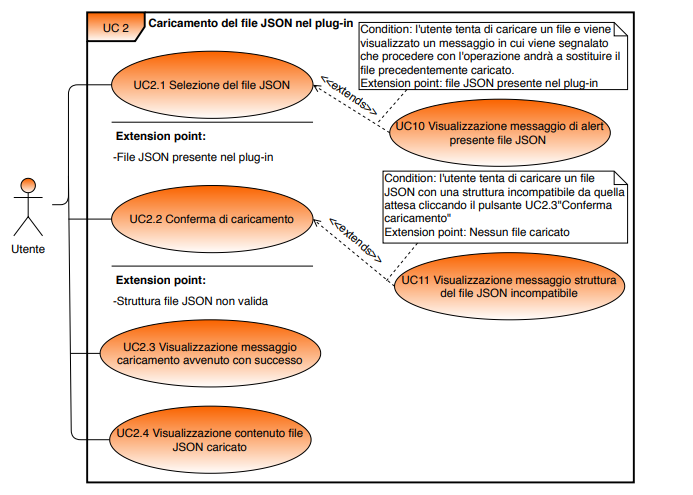
\includegraphics[scale=0.70]{../Analisi_dei_requisiti/img/Diagrammi_UML/UC2_Caricamento_file_JSON_nel_plug-in.png}
		\caption{Caricamento del file JSON}
	\end{figure}	
		
		\begin{itemize}
			\item\textbf{Attore primario}: utente generico;
			\item\textbf{Precondizioni}:
				\begin{enumerate}
					\item l'utente ha effettuato l'accesso alla piattaforma Grafana;
					\item l'utente ha selezionato una dashboard e ha aggiunto il plug-in “Predire in Grafana”, che verrà visualizzato sul rispettivo pannello;
					\item l'utente dispone del file JSON contenente i predittori (\hyperref[par:UC1]{UC1}).
				\end{enumerate}
			\item\textbf{Postcondizioni}:
				\begin{enumerate}
					\item l'utente ha caricato il file JSON con predittori associati nel plug-in;
					\item viene letta la definizione del predittore dal file in formato JSON.
				\end{enumerate}
			\item\textbf{Scenario principale}:
				\begin{enumerate}
					\item (\hyperref[par:UC2.1]{UC2.1}) l'utente seleziona il file JSON contenente i predittori da locale;
					\item (\hyperref[par:UC2.2]{UC2.2}) l'utente conferma il caricamento;
					\item (\hyperref[par:UC2.3]{UC2.3}) viene visualizzato a schermo un messaggio di notifica di avvenuto successo della procedura di caricamento JSON.
				\end{enumerate}
			\item\textbf{Estensioni}:
				\begin{enumerate}
					\item\hyperref[par:UC10]{UC10} estende \hyperref[par:UC2.1]{UC2.1}: viene visualizzato un messaggio di alert nel caso in cui sia già presente un file JSON caricato nel plug-in "Predire in Grafana";
					\item\hyperref[par:UC11]{UC11} estende \hyperref[par:UC2.2]{UC2.2}: viene visualizzato un messaggio d'errore nel caso in cui l'operazione di caricamento del file non sia andata a buon fine.
				\end{enumerate}	
			
		\end{itemize}
		
		
		\label{par:UC2.1}
		\subsubsection{UC2.1 - Selezione del file JSON}
		\begin{itemize}
			\item\textbf{Attore primario}: utente generico;
			\item\textbf{Precondizioni}:
				\begin{enumerate}
					\item l'utente visualizza il pannello “Predire in Grafana” nella dashboard;
					\item l'utente ha cliccato il pulsante "Carica JSON" e visualizza il pannello di selezione del file.
			\item\textbf{Postcondizioni}: l'utente ha selezionato il file JSON;
			\item\textbf{Scenario principale}: l'utente seleziona dalla finestra di selezione il file JSON da importare tra quelli disponibili e sono visibili solo i file con formato .json;
			\item\textbf{Estensioni}: \hyperref[par:UC10]{UC10}: viene visualizzato un messaggio di alert nel caso in cui sia già presente un file JSON caricato nel plug-in "Predire in Grafana".
				\end{enumerate}
			\end{itemize}
		
		\label{par:UC2.2}
		\subsubsection{UC2.2 - Conferma di caricamento}
		\begin{itemize}
			\item\textbf{Attore primario}: utente generico;
			\item\textbf{Precondizioni}: l'utente ha selezionato il file JSON da caricare;
			\item\textbf{Postcondizioni}: l'utente ha caricato il file nel plug-in;
			\item\textbf{Scenario principale}: l'utente clicca il pulsante etichettato con “Conferma” e il file viene caricato;
			\item\textbf{Estensioni}: \hyperref[par:UC11]{UC11}: viene visualizzato un messaggio d'errore nel caso in cui l'operazione di caricamento del file non sia andata a buon fine.
					
		\end{itemize}
		
		\label{par:UC2.3}
	\subsubsection{UC2.3 - Visualizzazione messaggio di notifica "Avvenuto successo caricamento JSON"}
		\begin{itemize}
			\item\textbf{Attore primario}: utente generico;
			\item\textbf{Precondizioni}: l'utente ha confermato il caricamento del file JSON selezionato (\hyperref[par:UC2.2]{UC2.2});
			\item\textbf{Postcondizioni}: l'utente visualizza la notifica di avvenuto caricamento del file JSON nel plug-in;
			\item\textbf{Scenario principale}:
				\begin{enumerate}
					\item l'utente visualizza il messaggio di notifica "Avvenuto successo caricamento file JSON" in cui viene notificato che il caricamento (\hyperref[par:UC2]{UC2}) è avvenuto correttamente;
					\item l'utente clicca il pulsante "Conferma" per proseguire.		
				\end{enumerate}		
		\end{itemize}

%%%%%%%%%%%%%%%%%%%%%%%%%%%%%%%

	\label{par:UC3}
	\subsection{UC3 - Collegamento del predittore al flusso dati}

		\begin{figure}[H]
		\centering
		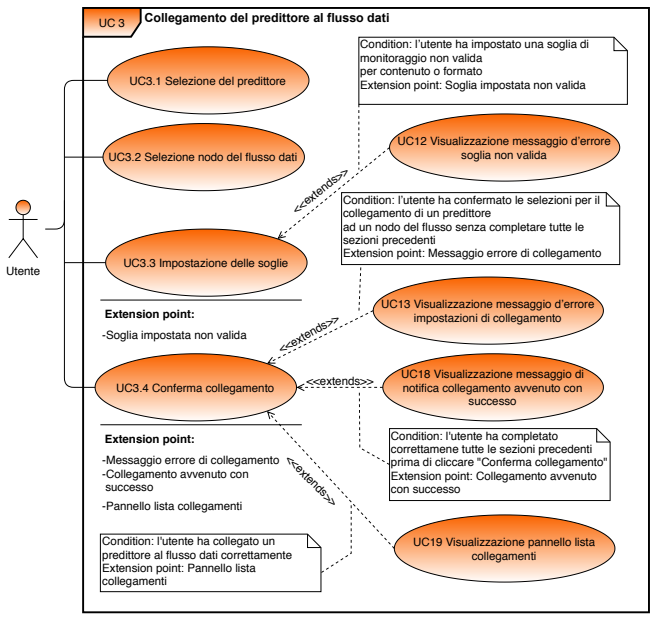
\includegraphics[scale=0.70]{../Analisi_dei_requisiti/img/Diagrammi_UML/UC3_collegamento_flusso_dati.png}
		\caption{Collegamento del predittore al flusso dati}
		\end{figure}	

		\begin{itemize}
			\item\textbf{Attore primario}: utente generico;
			\item\textbf{Precondizioni}:
				\begin{enumerate}
					\item l'utente ha caricato e letto con successo i predittori contenuti nel file JSON (\hyperref[par:UC2]{UC2});
					\item l'utente dispone di una serie di predittori da poter collegare al flusso di dati voluto;
					\item l'utente deve aver configurato la connessione al server tramite Grafana;
					\item l'utente deve disporre di almeno un database caricato in Grafana.	
				\end{enumerate}
			\item\textbf{Postcondizioni}: l'utente ha collegato correttamente i predittori ad un flusso dati, definendone le soglie per i rispettivi stati di ogni nodo e visualizza i collegamenti in un pannello dedicato;
			\item\textbf{Scenario principale}:
				\begin{enumerate}
					\item (\hyperref[par:UC3.1]{UC3.1}) l'utente seleziona uno o più predittori scegliendoli tra quelli disponibili in una lista che verrà visualizzata una volta caricato il file JSON;
					\item (\hyperref[par:UC3.2]{UC3.2}) l'utente seleziona il nodo del flusso dati da associare al predittore attraverso una query\glo;
					\item (\hyperref[par:UC3.3]{UC3.3}) impostazione delle soglie;
					\item (\hyperref[par:UC3.4]{UC3.4}) l'utente conferma le impostazioni di collegamento selezionate;	
					\item (\hyperref[par:UC3.5]{UC3.5}) viene visualizzata una notifica avvenuto collegamento al nodo del flusso dati se la procedura è andata a buon fine;
					\item (\hyperref[par:UC3.6]{UC3.6}) l'utente visualizza una lista dei collegamenti con le rispettive impostazioni di collegamento selezionate.
				\end{enumerate}
			\item\textbf{Estensioni}:
				\begin{enumerate}
					\item\hyperref[par:UC12]{UC12} estende \hyperref[par:UC3.3]{UC3.3}: viene visualizzato un messaggio di errore soglia non valida nel caso venga inserito un valore non consentito;
					\item\hyperref[par:UC13]{UC13} estende \hyperref[par:UC3.4]{UC3.4}: viene visualizzato un messaggio d'errore nel caso il collegamento non sia stato possibile.
						
				\end{enumerate}
		\end{itemize}
		

		\label{par:UC3.1}
		\subsubsection{UC3.1 - Selezione del predittore}
		\begin{itemize}
			\item\textbf{Attore primario}: utente generico;
			\item\textbf{Precondizioni}: è stato letto il file JSON con i predittori e l'utente visualizza una lista con i predittori disponibili;
			\item\textbf{Postcondizioni}: uno o più predittori sono stati selezionati dalla lista disponibile;
			\item\textbf{Scenario principale}: l'utente seleziona il predittore che intende associare ad un aspetto del flusso.
		\end{itemize}
		
	
	\label{par:UC3.2}
	\subsubsection{UC3.2 - Selezione nodo del flusso dati}
		\begin{itemize}
			\item\textbf{Attore primario}: utente generico;
			\item\textbf{Precondizioni}:
				\begin{enumerate}
					\item il predittore da collegare è stato selezionato dalla lista dei predittori (\hyperref[par:UC3.1]{UC3.1});
					\item sono state aggiunte delle query al sistema di Grafana;
					\item l'utente visualizza la lista di nodi del flusso di dati a cui poter associare il/i predittore/i selezionato/i.
				\end{enumerate}
			\item\textbf{Postcondizioni}: l'utente ha selezionato il nodo dal flusso dati;
			\item\textbf{Scenario principale}: l'utente seleziona l'aspetto interessato dal flusso di dati al quale può essere agganciato il predittore selezionato (o i predittori).
		\end{itemize}

	\label{par:UC3.3}
	\subsubsection{UC3.3 - Impostazione delle soglie}
		\begin{itemize}
			\item\textbf{Attore primario}: utente generico;
			\item\textbf{Precondizioni}: l'utente ha selezionato almeno un predittore che vuole collegare al flusso dati (\hyperref[par:UC3.1]{UC3.1});
			\item\textbf{Postcondizioni}: l'utente ha impostato la soglia di monitoraggio sul predittore selezionato;
			\item\textbf{Scenario principale}: l'utente dispone di almeno un predittore e aggiunge una soglia da associare; è possibile impostare più di una soglia;
			\item\textbf{Estensioni}: \hyperref[par:UC12]{UC12}: viene visualizzato un messaggio di errore "Soglia Non Valida" nel caso venga inserito un valore non consentito.
		\end{itemize}

	\label{par:UC3.4}
	\subsubsection{UC3.4 - Conferma collegamento}
		\begin{itemize}
			\item\textbf{Attore primario}: utente generico;
			\item\textbf{Precondizioni}: l'utente ha creato le basi per l'associazione del predittore al nodo del flusso dati scelto; in particolare è stato selezionato il predittore (\hyperref[par:UC3.1]{UC3.1}), il nodo del flusso dati da associare (\hyperref[par:UC3.2]{UC3.2}) ed è stata impostata una soglia (\hyperref[par:UC3.3]{UC3.3});
			\item\textbf{Postcondizioni}:
				\begin{enumerate}
					\item l'utente ha confermato il collegamento e visualizza la lista dei collegamenti;
					\item l'utente ha la possibilità di effettuare un altro collegamento tornando a \hyperref[par:UC3.1]{UC3.1}.
				\end{enumerate}
			\item\textbf{Scenario principale}: l'utente clicca il pulsante etichettato con "Conferma Collegamento";
			\item\textbf{Estensioni}: \hyperref[par:UC13]{UC13}: viene visualizzato un messaggio d'errore nel caso il collegamento non sia stato possibile.		
				
		\end{itemize}
		
	\label{par:UC3.5}
	\subsection{UC3.5 - Visualizzazione messaggio di notifica "Collegamento avvenuto con successo"}
		\begin{itemize}
			\item\textbf{Attore primario}: utente generico;
			\item\textbf{Precondizioni}: l'utente ha confermato il collegamento (\hyperref[par:UC3.4]{UC3.4});
			\item\textbf{Postcondizioni}: l'utente visualizza la notifica di avvenuto successo del collegamento;
			\item\textbf{Scenario principale}:
				\begin{enumerate}
					\item l'utente visualizza il messaggio di notifica "Collegamento avvenuto con successo" in cui viene notificato che il collegamento tra predittore e flusso dati (\hyperref[par:UC3]{UC3}) è avvenuto correttamente;
					\item l'utente clicca il pulsante "Conferma" per proseguire.		
				\end{enumerate}		
		\end{itemize}

	\label{par:UC3.6}
	\subsection{UC3.6 - Visualizzazione pannello lista collegamenti}
		\begin{itemize}
			\item\textbf{Attore primario}: utente generico;
			\item\textbf{Precondizioni}: l'utente ha confermato il collegamento tra predittore e nodo del flusso selezionato cliccando il pulsante di "Conferma collegamento" (\hyperref[par:UC3.4]{UC3.4});
			\item\textbf{Postcondizioni}: l'utente visualizza un pannello contenente la lista di tutti i collegamenti effettuati, ogni nuovo collegamento confermato viene aggiunto alla lista;
			\item\textbf{Scenario principale}:
				\begin{enumerate}
					\item l'utente visualizza la lista di collegamenti effettuati correttamente fino a quel momento; ogni riga è così suddivisa:
					\begin{itemize}
						\item nominativo del predittore (o predittori) selezionato;
						\item nominativo del nodo del flusso dati selezionato;
						\item impostazioni delle soglie inserite.
					\end{itemize}
					\item accanto ad ogni riga della lista dei collegamenti sono presenti i pulsanti "Scollega predittore" e "Modifica collegamento" .	
				\end{enumerate}		
		\end{itemize}


%%%%%%%%%%%%%%%%%%%%%%%%%%%%%%%

	\label{par:UC4}
	\subsection{UC4 - Operazioni sui collegamenti}

		\begin{figure}[H]
		\centering
		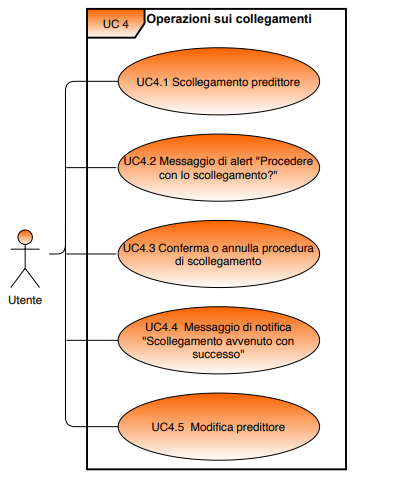
\includegraphics[scale=0.80]{../Analisi_dei_requisiti/img/Diagrammi_UML/UC4_Operazioni_sui_collegamenti.png}
		\caption{Operazioni sui collegamenti}
		\end{figure}	

		\begin{itemize}
			\item\textbf{Attore primario}: utente generico;
			\item\textbf{Precondizioni}:
				\begin{enumerate}
					\item l'utente si trova sul pannello dedicato alla lista dei collegamenti tra predittore e flusso dati (\hyperref[par:UC3.6]{UC3.6});
					\item la lista dei collegamenti presenta almeno un collegamento eseguito con successo (\hyperref[par:UC3]{UC3}).
				\end{enumerate}
			\item\textbf{Postcondizioni}:
				\begin{enumerate}
					\item l'utente ha scollegato il predittore dal nodo del flusso dati precedentemente associato oppure ha modificato il collegamento desiderato;
					\item se è avvenuto uno scollegamento dalla lista dei collegamenti non viene più visualizzato il collegamento che è stato scollegato.
				\end{enumerate}
			\item\textbf{Scenario principale}: 
			\begin{enumerate} 
				\item (\hyperref[par:UC4.1]{UC4.1}) l'utente clicca il pulsante con etichetta "Scollega predittore";
				\item (\hyperref[par:UC4.2]{UC4.2}) viene visualizzato un messaggio di alert "Procedere con lo scollegamento?" che interroga l'utente sull'effettiva conferma della procedura attuata;
				\item (\hyperref[par:UC4.3]{UC4.3}) l'utente clicca il pulsante "Conferma" per proseguire e scollegare il predittore oppure clicca il pulsante "Annulla" per ritornare alla lista dei collegamenti;	
				\item (\hyperref[par:UC4.4]{UC4.4}) viene visualizzato un messaggio di notifica "Scollegamento avvenuto con successo";
				\item (\hyperref[par:UC4.5]{UC4.5}) l'utente clicca il pulsante con etichetta "Modifica predittore";
			\end{enumerate}
	\end{itemize}
		
	\label{par:UC4.1}
	\subsubsection{UC4.1 - Scollegamento predittore}
		\begin{itemize}
			\item\textbf{Attore primario}: utente generico;
			\item\textbf{Precondizioni}: l'utente visualizza la lista dei collegamenti in cui è presente almeno un collegamento tra predittore e flusso dati;
			\item\textbf{Postcondizioni}: l'utente ha cliccato il pulsante di scollegamento;
			\item\textbf{Scenario principale}: l'utente clicca il pulsante con etichetta “Scollega predittore”;
			\end{itemize}
		
	\label{par:UC4.2}
	\subsubsection{UC4.2 - Visualizzazione messaggio di alert "Procedere con lo scollegamento"}
		\begin{itemize}
			\item\textbf{Attore primario}: utente generico;
			\item\textbf{Precondizioni}: l'utente ha selezionato il pulsante di scollegamento "Scollega predittore" (\hyperref[par:UC4.1]{UC4.1});
			\item\textbf{Postcondizioni}: l'utente ha visualizzato il messaggio di alert sul tentativo di scollegamento predittore;
					
			\item\textbf{Scenario principale}: l'utente visualizza un messaggio di alert "Procedere con lo scollegamento?" in cui viene segnalato che è stata selezionata una procedura di scollegamento del predittore.
	
		\end{itemize}		
		
	\label{par:UC4.3}
	\subsubsection{UC4.3 - Conferma scollegamento}
		\begin{itemize}
			\item\textbf{Attore primario}: utente generico;
			\item\textbf{Precondizioni}: l'utente ha visualizzato il messaggio di alert sul tentativo di scollegamento predittore;
			\item\textbf{Postcondizioni}: l'utente ha confermato o annullato la procedura di scollegamento;	
			\item\textbf{Scenario principale}: l'utente clicca il pulsante "Conferma" per proseguire e scollegare il predittore oppure clicca il pulsante "Annulla" per ritornare alla lista dei collegamenti.
			\end{itemize}
			
	\label{par:UC4.4}
	\subsubsection{UC4.4 - Visualizzazione messaggio di notifica "Scollegamento avvenuto con successo"}
		\begin{itemize}
			\item\textbf{Attore primario}: utente generico;
			\item\textbf{Precondizioni}: 
				\begin{enumerate}
					\item l'utente ha confermato lo scollegamento del predittore (\hyperref[par:UC4.3]{UC4.3})
				\end{enumerate}
			\item\textbf{Postcondizioni}: l'utente visualizza la notifica di scollegamento avvenuto con successo;					
			\item\textbf{Scenario principale}:
				\begin{enumerate}
					\item l'utente visualizza il messaggio di notifica "Scollegamento avvenuto successo" in cui viene notificato che lo scollegamento confermato(\hyperref[par:UC4.4]{UC4.4}) del predittore selezionato è avvenuto correttamente;
					\item l'utente clicca il pulsante "Conferma" per proseguire.		
				\end{enumerate}		
		\end{itemize}
			
	\label{par:UC4.5}
	\subsubsection{UC4.5 - Modifica collegamento}

		\begin{itemize}
			\item\textbf{Attore primario}: utente generico;
			\item\textbf{Precondizioni}: l'utente deve aver selezionato il collegamento che desidera modificare;
			\item\textbf{Postcondizioni}:
				\begin{enumerate}
					\item l'utente ha cliccato il tasto di modifica e viene indirizzato al pannello di collegamento del predittore al flusso dati a partire dalla sezione dedicata alla "Selezione del predittore" (\hyperref[par:UC3.1]{UC3.1}) dove può apportare le modifiche al collegamento scelto;
					\item la precedente selezione verrà evidenziata con un marcatore e verranno visualizzati i precedenti inserimenti; sarà possibile la modifica.
				\end{enumerate}
			\item\textbf{Scenario principale}:
				\begin{enumerate}
					\item l'utente clicca il pulsante "Modifica collegamento" e viene indirizzato alla sezione di "Selezione del predittore" (\hyperref[par:UC3.1]{UC3.1});
					\item vengono abilitate le modifiche e marcate le selezioni precedentemente effettuate. L'utente decide come modificare il collegamento reiterando le procedure di selezione del predittore (\hyperref[par:UC3.1]{UC3.1}), nodo del flusso dati (\hyperref[par:UC3.2]{UC3.2}), impostazione soglie (\hyperref[par:UC3.3]{UC3.3}) e conferma (\hyperref[par:UC3.4]{UC3.4}).
				\end{enumerate}		
		\end{itemize}

%%%%%%%%%%%%%%%%%%%%%%%%%%%%%%%

	\label{par:UC5}
	\subsection{UC5 - Operazioni calcolo di previsione}

	\begin{figure}[H]
		\centering
		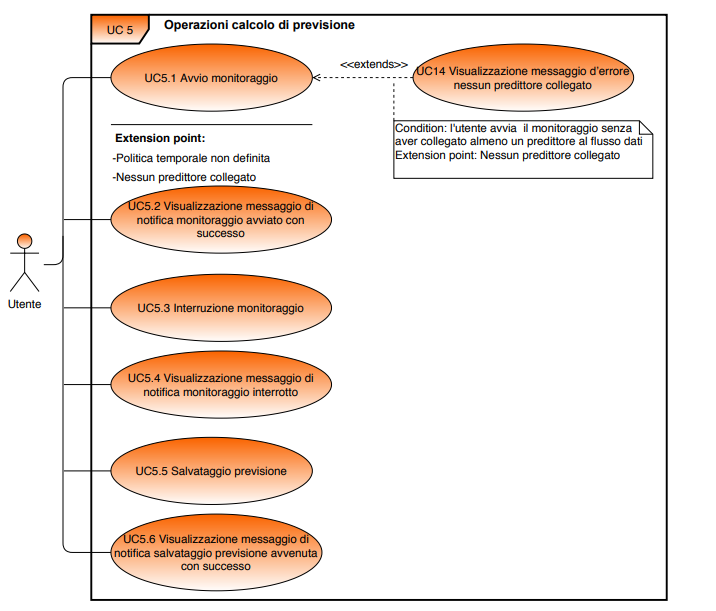
\includegraphics[scale=0.70]{../Analisi_dei_requisiti/img/Diagrammi_UML/UC5_Operazioni_calcolo_di_previsione.png}
		\caption{Operazioni sul calcolo di previsione}
	\end{figure}	

		\begin{itemize}
			\item\textbf{Attore primario}: utente generico;
			\item\textbf{Precondizioni}:
				\begin{enumerate}
					\item l'utente si trova nel pannello "Calcolo di previsione" relativo alle operazioni sulla previsione del flusso dati;
					\item è stato effettuato almeno un collegamento tra predittore e flusso dati da monitorare (\hyperref[par:UC3]{UC3}).
				\end{enumerate}		
	\item\textbf{Postcondizioni}:
				\begin{enumerate}
					\item è stata applicata la previsione al flusso di dati preso in esame ed è stato avviato il monitoraggio;
					\item è stato deciso se inviare o meno i nuovi dati a Grafana ottenuti dalla previsione.
				\end{enumerate}
			\item\textbf{Scenario principale}:
				\begin{enumerate}
					\item (\hyperref[par:UC5.1]{UC5.1}) l'utente inserisce la politica temporale\glo da applicare;
					\item (\hyperref[par:UC5.2]{UC5.2}) l'utente clicca il pulsante di avvio monitoraggio;
					\item (\hyperref[par:UC5.3]{UC5.3}) viene visualizzato un messaggio di notifica di "Monitoraggio avviato con successo";
					\item (\hyperref[par:UC5.4]{UC5.4}) una volta avviato il monitoraggio è possibile interromperlo cliccando il pulsante di interruzione.
					\item (\hyperref[par:UC5.5]{UC5.5}) viene visualizzata una notifica di "Monitoraggio interrotto";		
					\item (\hyperref[par:UC5.6]{UC5.6}) l'utente decide se salvare i dati di previsione cliccando il pulsante di salvataggio.
					\item (\hyperref[par:UC5.7]{UC5.7}) viene visualizzata un messaggio di notifica di "Invio dati avvenuto con successo";
				\end{enumerate}
			\item\textbf{Estensioni}:
				\begin{enumerate}
					\item \hyperref[par:UC14]{UC14} estende \hyperref[par:UC5.2]{UC5.2}: visualizzazione messaggio d'errore "Politica temporale non definita";
					\item \hyperref[par:UC15]{UC15} estende \hyperref[par:UC5.2]{UC5.2}: visualizzazione messaggio d'errore "Nessun predittore collegato".

				\end{enumerate}
		\end{itemize}

	
	\label{par:UC5.1}
	\subsubsection{UC5.1 - Inserimento politica temporale}
		\begin{itemize}
			\item\textbf{Attore primario}: utente generico;
			\item\textbf{Precondizioni}: l'utente si trova nella sezione "Calcolo di previsione" del pannello del plug-in;
			\item\textbf{Postcondizioni}: l'utente avrà selezionato una politica temporale applicabile ad un successivo calcolo di previsione;
			\item\textbf{Scenario principale}: l'utente inserisce il tempo di previsione sul flusso dati attraverso l'inserimento dei campi "Secondi", "Minuti", "Ore" nell'apposito spazio di editing.
		\end{itemize}	

	\label{par:UC5.2}
	\subsubsection{UC5.2 - Avvio monitoraggio}
		\begin{itemize}
			\item\textbf{Attore primario}: utente generico;
			\item\textbf{Precondizioni}: l'utente ha impostato la Politica Temporale (\hyperref[par:UC5.1]{UC5.1});
			\item\textbf{Postcondizioni}:
				\begin{enumerate}
					\item l'utente ha avviato il monitoraggio sul flusso dati cliccando sul pulsante di avvio;
					\item il bottone “Avvio monitoraggio” viene rimpiazzato da “Interruzione monitoraggio”;
					\item fino all'interruzione del monitoraggio l'utente non ha la possibilità di modificare i vari collegamenti.
				\end{enumerate}
			\item\textbf{Scenario principale}: l'utente avvia il calcolo di previsione selezionando il pulsante “Avvia monitoraggio”;
			\item\textbf{Estensioni}:
				\begin{enumerate}
					\item \hyperref[par:UC14]{UC14}: visualizzazione messaggio d'errore "Politica temporale non definita";
					\item \hyperref[par:UC15]{UC15}: visualizzazione messaggio d'errore "Nessun predittore collegato";
				\end{enumerate}
			
				
		\end{itemize}	
		
		\label{par:UC5.3}
	\subsubsection{UC5.3 - Visualizzazione messaggio di notifica "Monitoraggio avviato con successo"}	
		\begin{itemize}
			\item\textbf{Attore primario}: utente generico;
			\item\textbf{Precondizioni}: l'utente ha avviato un monitoraggio (\hyperref[par:UC5.2]{UC5.2});
			\item\textbf{Postcondizioni}: l'utente ha visualizzato la notifica di monitoraggio avviato con successo;
			\item\textbf{Scenario principale}:
				\begin{enumerate}
					\item l'utente visualizza il messaggio di notifica "Monitoraggio avviato con successo" in cui viene notificato che il monitoraggio è stato avviato correttamente;
					\item l'utente clicca il pulsante "Conferma" per proseguire.		
				\end{enumerate}		
		\end{itemize}
		
		\label{par:UC5.4}
	\subsubsection{UC5.4 - Interruzione monitoraggio}
		\begin{itemize}
			\item\textbf{Attore primario}: utente generico;
			\item\textbf{Precondizioni}: l'utente ha avviato il monitoraggio (\hyperref[par:UC5.2]{UC5.2});
			\item\textbf{Postcondizioni}:
				\begin{enumerate}
					\item l'utente ha deciso di interrompere il monitoraggio avviato precedentemente;
					\item il bottone “Interruzione monitoraggio” viene rimpiazzato da “Avvio monitoraggio”;
					\item l'utente ha nuovamente la possibilità di modificare i vari collegamenti.
				\end{enumerate}	
			\item\textbf{Scenario principale}: l'utente clicca il pulsante con etichetta “Interrompi monitoraggio” presente sul pannello di visualizzazione dei collegamenti;
			
		\end{itemize}

	\label{par:UC5.5}
	\subsubsection{UC5.5 - Visualizzazione messaggio di notifica "Monitoraggio interrotto"}
		\begin{itemize}
			\item\textbf{Attore primario}: utente generico;
			\item\textbf{Precondizioni}: l'utente ha interrotto il monitoraggio (\hyperref[par:UC5.4]{UC5.4});
			\item\textbf{Postcondizioni}: l'utente ha visualizzato la notifica di monitoraggio interrotto;
			\item\textbf{Scenario principale}:
				\begin{enumerate}
					\item l'utente visualizza il messaggio di notifica "Monitoraggio interrotto" in cui viene notificato che il monitoraggio sul flusso dati è stato interrotto;
					\item l'utente clicca il pulsante "Conferma" per proseguire.		
				\end{enumerate}		
		\end{itemize}
		
	\label{par:UC5.6}
	\subsubsection{UC5.6 - Salvataggio previsione}
		\begin{itemize}
			\item\textbf{Attore primario}: utente generico;
			\item\textbf{Precondizioni}:
				\begin{enumerate}
					\item è stata configurata correttamente la connessione al server tramite Grafana;
					\item l'utente ha avviato il monitoraggio (\hyperref[par:UC5.2]{UC5.2}) e dispone delle previsioni sul flusso di dati in quanto il calcolo di previsione è stato completato correttamente (\hyperref[par:UC5.3]{UC5.3}).
				\end{enumerate}
			\item\textbf{Postcondizioni}: la previsione calcolata sui dati ricevuti è stata immagazzinata nel DB se lo desidera;
			\item\textbf{Scenario principale}: l'utente clicca il pulsante “Invia previsioni” tramite il quale i dati di previsione vengono inviati al Database InfluxDB, altrimenti decide di non salvarli e prosegue con il monitoraggio.
			
		\end{itemize}	
		
	\label{par:UC5.7}
	\subsubsection{UC5.7 - Visualizzazione messaggio di notifica "Salvataggio previsione avvenuta con successo"}	\begin{itemize}
			\item\textbf{Attore primario}: utente generico;
			\item\textbf{Precondizioni}: l'utente ha cliccato il pulsante di invio previsioni (\hyperref[par:UC5.6]{UC5.6});
			\item\textbf{Postcondizioni}: l'utente ha visualizzato la notifica di "Salvataggio dati di previsione avvenuto con successo";
			\item\textbf{Scenario principale}:
				\begin{enumerate}
					\item l'utente visualizza il messaggio di notifica "Salvataggio previsione avvenuto con successo" in cui viene notificato che i dati di previsione sono stati inviati al Database (\hyperref[par:UC5.6]{UC5.6});
					\item l'utente clicca il pulsante "Conferma" per proseguire.		
				\end{enumerate}		
		\end{itemize}


%%%%%%%%%%%%%%%%%%%%%%%%%%%%%%%

	\label{par:UC6}
	\subsection{UC6 - Visualizzazione della dashboard}

	\begin{figure}[H]
		\centering
		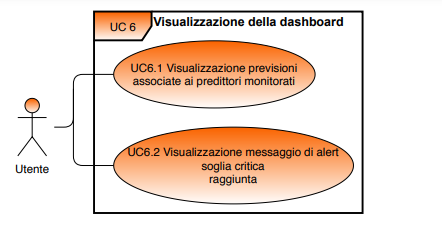
\includegraphics[scale=0.80]{../Analisi_dei_requisiti/img/Diagrammi_UML/UC6_Visualizzazione_della_dashboard.png}
		\caption{Visualizzazione delle previsioni}
	\end{figure}

		\begin{itemize}
			\item\textbf{Attore primario}: utente generico;
			\item\textbf{Precondizioni}: 
			\begin{enumerate}
				\item l'utente visualizza la dashboard a cui è stato aggiunto il plugin "Predire In Grafana";
				\item l'utente ha avviato correttamente il monitoraggio del flusso dati (\hyperref[par:UC5.2]{UC5.2}) con relativi predittori collegati.
			\end{enumerate}				
			\item\textbf{Postcondizioni}: il sistema mantiene aggiornate e visualizzabili attraverso l'uso delle dashboard le misurazioni e le previsioni dei predittori associati da parte dell'utente;
			\item\textbf{Scenario principale}: 
			\begin{enumerate}
				\item (\hyperref[par:UC6.1]{UC6.1}) l'utente visualizza le previsioni calcolate nella dashboard di Grafana;
				\item (\hyperref[par:UC6.2]{UC6.2}) ogni volta che una soglia critica viene attivata dai dati di previsioni viene visualizzato un messaggio di alert.
			\end{enumerate}
				
		\end{itemize}
		
		\label{par:UC6.1}
	\subsection{UC6.1 - Visualizzazione previsioni}
		\begin{itemize}
			\item\textbf{Attore primario}: utente generico;
			\item\textbf{Precondizioni}: l'utente ha avviato correttamente il monitoraggio del flusso dati (\hyperref[par:UC5.3]{UC5.3}) con relativi predittori collegati;
			\item\textbf{Postcondizioni}: l'utente ha visualizzato sulla dashboard le previsioni calcolate precedentemente;
			\item\textbf{Scenario principale}: l'utente visualizza le previsioni calcolate. Il sistema si aggiorna costantemente grazie ai dati provenienti dal database, effettuando l'operazione di calcolo delle previsioni sul flusso dati associato ai predittori (\hyperref[par:UC5]{UC5}). Tale operazione di calcolo di previsione viene eseguito in base alla politica temporale stabilita in \hyperref[par:UC5.1]{UC5.1};	
		\end{itemize}
			
		
		\label{par:UC6.2}
	\subsection{UC6.2 - Visualizzazione messaggio di alert "Soglia critica raggiunta"}
		\begin{itemize}
			\item\textbf{Attore primario}: utente generico;
			\item\textbf{Precondizioni}: una delle soglie impostate per il predittore (\hyperref[par:UC3.3]{UC3.3}) è stata raggiunta o superata;
			\item\textbf{Postcondizioni}: l'utente ha visualizzato il messaggio di alert riguardante la soglia interessata;
			\item\textbf{Scenario principale}:
				\begin{enumerate}
					\item l'utente visualizza il messaggio di alert "Soglia critica raggiunta" in cui viene segnalato che una soglia impostata nel processo di collegamento dei predittori al flusso dati (\hyperref[par:UC3.3]{UC3.3}) è stata raggiunta o superata;
					\item l'utente clicca il pulsante "Conferma" per proseguire.		
				\end{enumerate}		
		\end{itemize}
	


% - Casi d'uso: Estensioni - %%%%%%%%%%%%%%%%%%%%%%%%%%%%%%%%%%%
	
	\label{par:UC7}
	\subsection{UC7 - Visualizzazione messaggio d'errore "Nessun file CSV caricato"}
		\begin{itemize}
			\item\textbf{Attore primario}: utente generico;
			\item\textbf{Precondizioni}: l'utente ha cliccato il pulsante di conferma (\hyperref[par:UC1.3]{UC1.3}) senza aver caricato un file CSV contenente i valori utilizzati per l'addestramento (\hyperref[par:UC1.1]{UC1.1});
			\item\textbf{Postcondizioni}: l'utente visualizza l'errore, viene quindi riportato alla finestra di selezione del file CSV (\hyperref[par:UC1.1]{UC1.1});
			\item\textbf{Scenario principale}: l'utente visualizza il messaggio d'errore "Nessun file CSV caricato" in cui viene segnalato il fatto che non è stato caricato alcun file CSV (\hyperref[par:UC1.1]{UC1.1}) e quindi non si può procedere con l'addestramento; 		
		\end{itemize}
		
	\label{par:UC8}
	\subsection{UC8 - Visualizzazione messaggio d'errore "Nessun algoritmo selezionato"}
		\begin{itemize}
			\item\textbf{Attore primario}: utente generico;
			\item\textbf{Precondizioni}: l'utente ha cliccato il pulsante di conferma (\hyperref[par:UC1.3]{UC1.3}) senza aver scelto un algoritmo dalla Combo Box (\hyperref[par:UC1.2]{UC1.2});
			\item\textbf{Postcondizioni}: l'utente visualizza l'errore, viene quindi riportato alla scelta dell'algoritmo (\hyperref[par:UC1.2]{UC1.2});
			\item\textbf{Scenario principale}: l'utente visualizza il messaggio d'errore "Nessun algoritmo selezionato" in cui viene segnalato il fatto che non è stato scelto alcun algoritmo da addestrare (\hyperref[par:UC1.2]{UC1.2}) e quindi non si può procedere con l'addestramento; 		
		\end{itemize}
	
	\label{par:UC9}
	\subsection{UC9 - Visualizzazione messaggio d'errore "File CSV incompatibile"}
		\begin{itemize}
			\item\textbf{Attore primario}: utente generico;
			\item\textbf{Precondizioni}: l'utente ha selezionato il file CSV che intende utilizzare per l'addestramento e ha cliccato il pulsante di conferma. Il file selezionato è strutturalmente errato e non c'è compatibilità con l'algoritmo selezionato;
			\item\textbf{Postcondizioni}: l'utente visualizza l'errore, viene quindi riportato alla finestra di selezione del file CSV (\hyperref[par:UC1.1]{UC1.1});
			\item\textbf{Scenario principale}: l'utente visualizza il messaggio d'errore "File incompatibile" in cui viene segnalato il fatto che il file CSV da lui selezionato (\hyperref[par:UC1.1]{UC1.1}) non è adatto per l'addestramento; 		
		\end{itemize}

%%%%%%%%%%%%%%%%%%%%%%%%%%%%%%%

	\label{par:UC10}
	\subsection{UC10 - Visualizzazione messaggio di alert "File JSON già caricato"}
		\begin{itemize}
			\item\textbf{Attore primario}: utente generico;
			\item\textbf{Precondizioni}: l'utente ha selezionato l'opzione di caricamento del file JSON tramite click del pulsante "Carica JSON" (\hyperref[par:UC2.1]{UC2.1});
			\item\textbf{Postcondizioni}: l'utente ha visualizzato un messaggio di alert in cui viene segnalato che è già presente un file JSON caricato nel plug-in;
			\item\textbf{Scenario principale}:
				\begin{enumerate}
					\item l'utente visualizza il messaggio di alert "File JSON già caricato" in cui viene segnalato che è già stato caricato un file JSON in precedenza e la conferma procederà alla sua sovrascrizione;
					\item l'utente clicca il pulsante "Conferma" per proseguire e caricare il nuovo file JSON oppure clicca il pulsante "Annulla" per ritornare alla sezione di caricamento.
				\end{enumerate}
		\end{itemize}	

%%%%%%%%%%%%%%%%%%%%%%%%%%%%%%%	

	\label{par:UC11}
	\subsection{UC11 - Visualizzazione messaggio d'errore "Caricamento file JSON" }
		\begin{itemize}
			\item\textbf{Attore primario}: utente generico;
			\item\textbf{Precondizioni}: l'utente ha selezionato il file JSON da caricare (\hyperref[par:UC2.1]{UC2.1}) e ha cliccato il pulsante di conferma (\hyperref[par:UC2.2]{UC2.2});
			\item\textbf{Postcondizioni}: l'utente ha visualizzato un messaggio d'errore in cui viene segnalato che la struttura del file selezionato non supporta una SVM o RL, di conseguenza viene riportato alla selezione del file JSON;
			\item\textbf{Scenario principale}:
				\begin{enumerate}
					\item l'utente visualizza il messaggio d'errore "Struttura del file JSON non supportata" in cui viene segnalato che la definizione dei predittori del file JSON selezionato (\hyperref[par:UC2.1]{UC2.1}) non è sintatticamente corretta;
					\item l'utente clicca il pulsante "Conferma" per proseguire e viene riportato alla sezione di selezione.
				\end{enumerate}
		\end{itemize}	

%%%%%%%%%%%%%%%%%%%%%%%%%%%%%%%

		\label{par:UC12}
	\subsection{UC12 - Visualizzazione messaggio d'errore "Soglia non valida"}
		\begin{itemize}
			\item\textbf{Attore primario}: utente generico;
			\item\textbf{Precondizioni}: l'utente ha impostato una soglia di monitoraggio(\hyperref[par:UC3.3]{UC3.3}) non valida per contenuto o formato;
			\item\textbf{Postcondizioni}: l'utente visualizza il messaggio d'errore sulla soglia appena impostata;		
			\item\textbf{Scenario principale}:
				\begin{enumerate}
					\item l'utente visualizza il messaggio d'errore "Errore Impostazione Soglia Non Valida" in cui viene segnalato che la soglia appena inserita (\hyperref[par:UC3.3]{UC3.3}) non può essere accettata e viene invitato ad inserirla nuovamente;
					\item l'utente clicca il pulsante "Conferma" per proseguire e viene riportato all'inserimento della soglia.		
				\end{enumerate}		
		\end{itemize}

%%%%%%%%%%%%%%%%%%%%%%%%%%%%%%%

	\label{par:UC13}
	\subsection{UC13 - Visualizzazione messaggio d'errore "Impostazioni di collegamento"}
		\begin{itemize}
			\item\textbf{Attore primario}: utente generico;
			\item\textbf{Precondizioni}: l'utente ha confermato le selezioni per il collegamento di un predittore ad un nodo del flusso (\hyperref[par:UC3.4]{UC3.4}) ed ha commesso alcuni errori;
			\item\textbf{Postcondizioni}:
				\begin{enumerate}
					\item l'utente visualizza il messaggio di errore di collegamento;
					\item le scelte dell'utente precedenti non vengono finalizzate e non viene creato il collegamento.
				\end{enumerate}		
			\item\textbf{Scenario principale}:
				\begin{enumerate}
					\item l'utente visualizza il messaggio d'errore "Errore impostazioni di collegamento" in cui viene segnalato che sono presenti errori o mancate selezioni nella procedura di collegamento (\hyperref[par:UC3]{UC3});
					\item l'utente clicca il pulsante "Conferma" per proseguire.		
				\end{enumerate}		
		\end{itemize}

%%%%%%%%%%%%%%%%%%%%%%%%%%%%%%%

		\label{par:UC14}
	\subsection{UC14 - Visualizzazione messaggio d'errore "Politica temporale non definita"}
		\begin{itemize}
			\item\textbf{Attore primario}: utente generico;
			\item\textbf{Precondizioni}: l'utente ha cliccato il pulsante di "Avvio monitoraggio" (\hyperref[par:UC5.2]{UC5.2}), senza aver impostato alcuna politica temporale per il calcolo di previsione (\hyperref[par:UC5.1]{UC5.1});
			\item\textbf{Postcondizioni}:
				\begin{enumerate}
					\item l'utente ha visualizzato il messaggio d'errore sulla politica temporale non definita;		
					\item	il monitoraggio non viene avviato.
				\end{enumerate}
			\item\textbf{Scenario principale}:
				\begin{enumerate}
					\item l'utente visualizza il messaggio d'errore "Errore politica temporale non definita" in cui viene segnalato che non è stata inserita nessuna politica temporale prima dell'avvio del monitoraggio;
					\item l'utente clicca il pulsante "Conferma" per proseguire e viene riportato all'inserimento della politica temporale (\hyperref[par:UC5.1]{UC5.1}).		
				\end{enumerate}		
		\end{itemize}

%%%%%%%%%%%%%%%%%%%%%%%%%%%%%%%
	
		\label{par:UC15}
	\subsection{UC15 - Visualizzazione messaggio d'errore "Nessun predittore collegato"}
		\begin{itemize}
			\item\textbf{Attore primario}: utente generico;
			\item\textbf{Precondizioni}: l'utente ha avviato il monitoraggio (\hyperref[par:UC5.2]{UC5.2}), senza aver impostato alcun collegamento (\hyperref[par:UC3]{UC3});
			\item\textbf{Postcondizioni}:
				\begin{enumerate}
					\item l'utente ha visualizzato il messaggio d'errore sulla mancata presenza di collegamenti;	
					\item	il monitoraggio non viene avviato.
				\end{enumerate}
			\item\textbf{Scenario principale}:
				\begin{enumerate}
					\item l'utente visualizza il messaggio d'errore "Nessun predittore collegato" in cui viene segnalato che non è stata inserito alcun collegamento tra predittore e flusso dati;
					\item l'utente clicca il pulsante "Conferma" per proseguire e viene riportato all'impostazione di collegamento predittori (\hyperref[par:UC3]{UC3}).		
				\end{enumerate}		
		\end{itemize}


	
%%%%%%%%%%%%%%%%%%%%%%%%%%%%%%%








